\documentclass{article}
\usepackage{graphicx, soul, parskip, amsmath, amssymb}
\usepackage[dvipsnames]{xcolor}
\usepackage[a4paper, margin=0.8in]{geometry}
\usepackage[spanish]{babel}

\setul{0.5ex}{0.3ex}

\newcommand{\ulcolor}[2][Red]{\setulcolor{#1}\ul{#2}}
\newcommand*\sepline{%
  \begin{center}
    \rule[1ex]{.5\textwidth}{.5pt}
  \end{center}}

\title{Ejercicios Adicionales $-$ Difíciles (Resuelto)}
\author{Juani Elosegui}
\date{Diciembre 2024}

\begin{document}
    
    \maketitle

    \section*{\underline{Ejercicio 1}}
        \begin{center}
            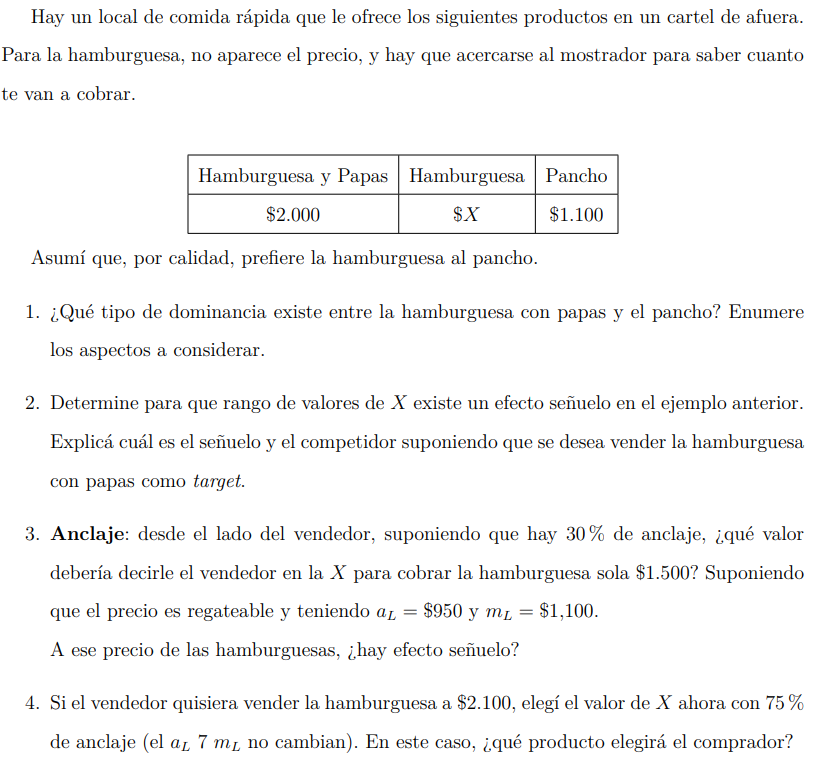
\includegraphics[width=0.8 \linewidth]{figs/adicionales-dificiles-uno.png}
        \end{center}
        \textbf{¿Qué tipo de dominancia existe entre la hamburguesa con papas y el pancho? Enumere los aspectos a considerar.}
        \\
        \\
        La hamburguesa con papas tiene una dominancia leve con respecto al pancho. La gente no siempre va a elegir la hamburguesa con papas, pero sí con una amplia mayoría.
        \\
        \\
        \textbf{Determine para que rango de valores de X existe un efecto señuelo en el ejemplo anterior. Explicá cuál es el señuelo y el competidor suponiendo que se desea vender la hamburguesa con papas como target.}
        \\
        \\
        Para un rango de valores de \(\mathdollar 1.100 < \mathdollar X < \mathdollar 2.000\) existe el efecto señuelo. El señuelo como tal es la hamburguesa, y su competidor es el pancho (ya que es la opción inicial del consumidor si no estuviera la hamburguesa).
        
\end{document}